\chapter{Sensor Fusion}
\section{Panoramica}
Nei sistemi in cui \`e richiesta un'alta \emph{reliability} delle misure, l'informazione fornita dai singoli sensori non \`e sufficiente. In questi casi \`e raccomandato l'utilizzo di un insieme di sensori in contemporanea.\\*
In un sistema che implementa SFA, ogni sensore \`e caratterizzato dal tipo dei suoi input e dei suoi output, dalla sua configurazione e dalle sue caratteristiche fisiche. Queste sorgenti eterogenee di dati devono essere integrate al fine di fornire le informazioni ricercate dalla particolare applicazione.\\*
SFA \`e considerato una famiglia di algoritmi di stima statistica, la scelta di un particolare algoritmo \`e legata alla particolare applicazione per cui si intende utilizzare SFA. Nel caso del posizionamento ferroviario si utilizza un algoritmo noto come Filtro di Kalman.
Esistono diversi tipi di Filtri di Kalman. Una prima classificazione viene fatta sulla base dell'architettura scelta, la quale pu\'o essere centralizzata o decentralizzata.\\*
In un'architettura centralizzata esiste un unico modulo che riceve in ingresso le misurazioni dei sensori e fornisce in uscita l'informazione ricercata. Questa architettura \`e schematizzabile come nella figura \ref{fig:sfa} mostrata nel Capitolo 1.\\*
Un'architettura decentralizzata diferisce dalla prima in quanto:
\begin{itemize}
	\item Esiste un sensore principale, detto \emph{main sensor};
	\item Le misure di ciascun sensore vengono processate assieme alla misura del \emph{main sensor} in sotto moduli, denominati \emph{local filters}, che implementano un Filtro di Kalman su un insieme ridotto di dati;
	\item Le uscite di ciascun \emph{local filter} vengono infine processate da un modulo denominato \emph{master filter}.
\end{itemize}
Ulteriori classificazioni vengono fatte su caratteristiche intrinseche dell'algoritmo implementato dal Filtro di Kalman.
\section{Misure e rumore}
Un Filtro di Kalman \`e utilizzato per stimare lo stato di un sistema dinamico in un ambiente caratterizzato da \emph{rumore}.
Un sistema dinamico \`e una modellazione matematica di un processo che evolve nel tempo, la cui evoluzione \`e descritta attraverso un sistema di equazioni differenziali o alle differenze, nel caso esso si evolva rispettivamente a tempo continuo o a tempo discreto.\\*
Senza perdere in generalit\`a, si possono formalizzare questi due tipi di sistemi dinamici come:
$$
y'(t) = f(t,y(t)),\;t\ge 0
$$
Con $y(0) \in \mathbb{R}^m$ condizione iniziale nota, e:
$$
y_{n+1} = f(n,y_n),\;n = 0,1,\dots
$$
con al solito $y_0 \in \mathbb{R}^m$ condizione iniziale nota.\\*
Ricavare lo stato del sistema dinamico per un certo istante $t$, o $n$, equivale a risolvere le equazioni cui sopra e valutarne la traiettoria soluzione in $t$ o in $n$.\\*
Un semplice sistema dinamico \`e rappresentato da un punto materiale che si muove con una accelerazione costante $$\vec{a} = a\vec{k}$$ dove $\vec{k}$ \`e un qualunque versore della base canonica di $\mathbb{R}^3$.\\*
Supponendo che il punto si muova con velocit\`a iniziale $\vec{z'}(0) = v_0\vec{k}$ nota e inizi il moto da una coordinata $\vec z(0) = z_0\vec{k}$ nota, si ha:
$$
z''(t) = a
$$
$$
z'(t) = \int{a dt} = a t + v_0
$$
$$
z(t) = \int(a t + v_0)dt = \frac{1}{2} at^2 +  v_0 t + z_0
$$
L'equazione $z(t)$ descrive completamente la traiettoria di moto del punto materiale, mentre $z'(t)$ descrive completamente la traiettoria della velocit\`a del punto durante il suo moto.\\*
In questo semplice esempio, viene fatta l'assunzione di conoscere a priori il valore esatto di $a$, di $v_0$ e di $z_0$.\\*
Nella pratica, per misurare l'accelerazione $a$ \`e necessario uno strumento denominato \emph{accelerometro}, il quale produrr\`a delle misure giocoforza affette da errori casuali. Si supponga di sostituire $a$ nell'equazione $z(t)$ con una sua perturbazione $\tilde{a} = a + \varepsilon$ dove $\varepsilon$ \`e una variazione casuale della misura data dal \emph{rumore} che caratterizza qualsiasi processo di misura. Si pu\'o supporre $Var(\varepsilon) = 0$ e considerare, ai fini di questa trattazione, $\varepsilon$ come un valore costante; in realt\`a $\varepsilon$ \`e una variable casuale a varianza generalmente non nulla. Si suppongano inoltre $v_0 = z_0 = 0$ per comodit\`a di calcolo:
$$
z(t) = \frac{1}{2} \tilde{a} t^2 = \frac{1}{2}(a + \varepsilon) t^2 = \frac{1}{2} \left(at^2 + \varepsilon t^2\right)
$$
Si nota immediatamente che la variazione della misura $z(t)$ data da $\varepsilon$ aumenta con il quadrato del tempo.\\*
\begin{figure}[h]
	\centering
	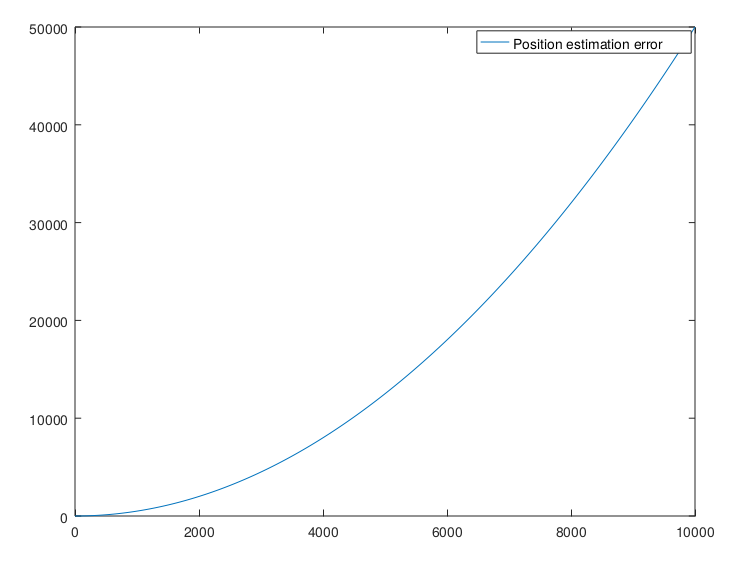
\includegraphics[scale=0.5]{img/errormeas}
	\caption{Grafico dell' errore di stima della posizione con $a = 10^0, \varepsilon = 10^{-3}$}
	\label{fig:errormeas}
\end{figure}
\noindent{}Un Filtro di Kalman \`e un modello progettato appositamente per risolvere o rendere trascurabile il problema del rumore nei processi di misura.\\*
Nel modellare un sistema dinamico complesso come il moto di un treno lungo una traccia ferroviaria, occorre tenere in considerazione le misure di accelerazione, velocit\`a, e posizione sia lineari che angolari. Tutte queste misurazioni saranno in generale caratterizzate da un rumore casuale che ne impedisce la corretta acquisizione, in quest'ottica \`e dunque fondamentale utilizzare un Filtro di Kalman. Per completezza di esposizione, occorre precisare che esistono anche fonti note e deterministiche di errore, oltre alle sorgenti casuali date dal rumore. Un Filtro di Kalman \`e in grado di rigettare una misurazione quando questa \`e affetta da un evidente errore deterministico, dello strumento o dell'operatore.
\section{Kalman Filtering}
Nell'applicare un Filtro di Kalman ad uno specifico sistema, devono essere noti i parametri del modello $\Phi,B,H$, il rumore statistico $(R,Q)$, il vettore delle condizioni iniziali $X_0$, e la sua matrice di covarianza $P_0$.\\*
Assumendo per semplicit\`a di avere un processo evolutivo a tempo discreto,
un Filtro di Kalman stima il vettore $X(n+1)$ che rappresenta lo stato del sistema al tempo $t+1$ con le informazioni disponibili al tempo $t$. Il filtro \`e dato da:
$$
P*_(n+1) = \Phi P_(n)\Phi^T + C
$$